\documentclass[12pt, a4paper]{report}
\usepackage[top=1cm, left=1cm, right=1cm]{geometry}

\usepackage[utf8]{inputenc}
\usepackage[russian]{babel}

\usepackage{array}
\newcolumntype{M}[1]{>{\centering\arraybackslash}m{#1}}

\usepackage{hyperref}
\hypersetup{
	colorlinks,
	citecolor=black,
	filecolor=black,
	linkcolor=black,
	urlcolor=black
}

\usepackage{sectsty}
\allsectionsfont{\centering}

\usepackage{indentfirst}
\setlength\parindent{24pt}

\usepackage{algorithm}
\usepackage[noend]{algpseudocode}

\usepackage{listings}
\usepackage{xcolor}
\definecolor{codegreen}{rgb}{0,0.6,0}
\definecolor{codegray}{rgb}{0.5,0.5,0.5}
\definecolor{codepurple}{rgb}{0.58,0,0.82}
\definecolor{backcolour}{rgb}{0.95,0.95,0.92}
\lstdefinestyle{mystyle}{
    backgroundcolor=\color{backcolour},   
    commentstyle=\color{codegreen},
    keywordstyle=\color{magenta},
    numberstyle=\normalsize\color{codegray},
    stringstyle=\color{codepurple},
    basicstyle=\ttfamily\footnotesize,
    breakatwhitespace=false,         
    breaklines=true,                 
    captionpos=b,                    
    keepspaces=true,                 
    numbers=left,                    
    numbersep=5pt,                  
    showspaces=false,                
    showstringspaces=false,
    showtabs=false,                  
    tabsize=2
}

\usepackage{graphicx}
\graphicspath{{plots/pictures/}}

\begin{document}
	\begin{titlepage}
		\begin{center}
			\large \textbf{Министерство науки и высшего образования Российской Федерации} \\
			\large \textbf{Федеральное государственное бюджетное образовательное учреждение высшего образования} \\
			\large \textbf{«Российский химико-технологический университет имени Д.И. Менделеева»} \\

			\vspace*{4cm}
			\LARGE \textbf{ОТЧЕТ ПО ЛАБОРАТОРНОЙ РАБОТЕ №1}

			\vspace*{4cm}
			\begin{flushright}
				\Large
				\begin{tabular}{>{\raggedleft\arraybackslash}p{9cm} p{10cm}}
					Выполнил студент группы КС-36: & Золотухин А.А. \\
					Ссылка на репозиторий: & https://github.com/ \\ 
					& MUCTR-IKT-CPP/ \\
					& ZolotukhinAA\_36\_ALG \\
					Принял: & Крашенников Роман Сергеевич \\
					Дата сдачи: & 17.02.2025 \\
				\end{tabular}

			\end{flushright}

			\vspace*{6cm}
			\Large \textbf{Москва \\ 2025}
		\end{center}
	\end{titlepage}
	
	\tableofcontents	
	\thispagestyle{empty}
	\newpage

	\pagenumbering{arabic}
	
	\section*{Описание задачи}
	\addcontentsline{toc}{section}{Описание задачи}
	\large
	В лабораторной работе предлагается изучить способ анализа алгоритма, связанный со временем. Рассмотреть для выбранного алгоритма сортировки наилучшее, наихудшее и среднее время и соотнести его с известным для алгоритма показателм эффективности O-большое. \par
	Допускается реализация задания на любом языке программирования, кроме лиспоподобных. Преподаватель может не знать конкретного языка реализации, поэтому вы должны быть способны объяснить алгоритм и нарисовать его без демонстрации непосредственно вашего кода. \par
	Задание:
	\begin{itemize}
		\item Реализовать метод сортировки: \textbf{Сортировка вставками};
		\item Реализовать проведения тестирования алгоритма сериями расчетов для измерения параметров За один расчёт выполняются следующие операции:
		\begin{itemize}
			\item Генерируется массив случайных значений;
			\item Запоминается время начала расчета алгоритма сортировки;
			\item Выполняется алгоритм сортировки
			\begin{itemize}
				\item Во время выполнения измерить количество повторных прохождений по массиву.
				\item Во время выполнения измерить количество выполнения операций обмена значений.
			\end{itemize}
			\item Вычисляется время, затраченное на сортировку: текущее время - время начала;
			\item Сохраняется время для одной попытки После этого расчёт повторяется до окончания серии.
			\begin{itemize}
				\item Алгоритм вычисляется 8 сериями по 20 раз за серию;
				\item Алгоритм в каждой серии вычисляется для массива размером M. (1000,2000, 4000, 8000, 16000, 32000, 64000, 128000);
				\item Массив заполняется значениями чисел с плавающей точкой в интервале от -1 до 1;
				\item Для серии запоминаются все времена, которые были замерены.
			\end{itemize}
		\end{itemize}
		\item По полученным данным времени построить графики зависимости времени от числа элементов в массиве:
		\begin{itemize}
			\item Совмещенный график наихудшего времени выполнения сортировки и сложности алгоритма, указанной в нотации O большое; \par
			Для построения графика вычисляется O большое для каждого размера массива. При этом при вычислении функции O(c * g(N)) подбирается такая константа c, чтобы при значении >1000 график O(N) был выше графика наихудшего случая, но второй график на его фоне не превращался в прямую линию.
			\item Совмещенный график среднего, наихудшего и наилучшего времени исполнения;
			\item График среднего количества обмена значений;
			\item График повторных обходов массива.
		\end{itemize}
		\item По результатам расчётов оформляется отчёт по предоставленной форме, в отчете:
		\begin{itemize}
			\item Приводится описание алгоритма;
			\item Приводится описание выполнения задачи (описание кода и специфических элементов реализации);
			\item Приводятся выводы (Графики и их анализ).
		\end{itemize}
	\end{itemize}

	\section*{Описание метода/модели}
	\addcontentsline{toc}{section}{Описание метода/модели}
	\large
	\textbf{Сортировка вставками} - это простой алгоритм сортировки, который работает путём итеративной вставки каждого элемента несортированного списка в его правильное положение в отсортированной части списка. Это похоже на сортировку игральных карт в ваших руках. Вы разделяете карты на две группы: отсортированные карты и несортированные карты. Затем вы выбираете карточку из несортированной группы и помещаете её в нужное место в отсортированной группе. \par
	Ход алгоритма:
	\begin{enumerate}
		\item Начинаем со второго элемента массива, поскольку предполагается, что первый элемент в массиве должен быть отсортирован;
		\item Сравниваем второй элемент с первым и проверяем, не меньше ли второй элемент, затем меняем их местами;
		\item Переходим к третьему элементу, сравниваем его с первыми двумя элементами и устанавливаем в правильное положение;
		\item Повторяем до тех пор, пока не будет отсортирован весь массив.
	\end{enumerate}
	Анализ сложности сортировки вставками:
	\begin{itemize}
		\item \textbf{Лучший вариант: O(\( N \))}, если список уже отсортирован;
		\item \textbf{Средний вариант: O(\( N^2 \))}, если список упорядочен случайным образом;
		\item \textbf{Наихудший вариант: O(\( N^2 \))}, если список находится в обратном порядке, \par
		где N - количество элементов в списке.
	\end{itemize}
	\begin{algorithm}
		\caption{Реализация алгоритма сортировки вставками}
		\begin{algorithmic}
			\State $i \gets 2$
			\While{$i \leq n - 1$}
				\State $j \gets i - 1$
				\While{$j \geq 0 AND A[j] > A[j + 1]$}
					\State $swap(A[j], A[j + 1])$
					\State $j \gets j - 1$
				\EndWhile
			\EndWhile
		\end{algorithmic}
	\end{algorithm}
	\textit{Преимущества}:
	\begin{itemize}
		\item Эффективно справляется с небольшими и почти отсортированными массивами;
		\item Экономит место;	
		\item Простой и легкореализуемый.
	\end{itemize}
	\textit{Недостатки}:
	\begin{itemize}
		\item Неэффективно справляется с большими массивами.
	\end{itemize}

	\section*{Выполнение задачи}
	\addcontentsline{toc}{section}{Выполнение задачи}
	Алгоритм сортировки вставками реализован на языке \textit{C++}. Построение графиков проводить с помощью программы \textit{GNUplot}.

	\textit{"main"} функция работает с циклом, в ходе которого производится расчёт минимального, максимального и среднего времени на сортировку массива размером \textit{M}. Каждая серия просчитывается по 20 раз. В итоге получаются данные, выведенные в определенные файлы, с помощью которых впоследствии строятся графики.
	\lstset{style=mystyle}
	\begin{lstlisting}[language=C++]
		int main() {
			std::ofstream worst_and_complexity(Constants::folder + "worst_and_complexity.dat");
			std::ofstream average_best_worst(Constants::folder + "average_best_worst.dat");
			std::ofstream average_swaps(Constants::folder + "average_swaps.dat");
			std::ofstream average_passes(Constants::folder + "average_passes.dat");
			if (!worst_and_complexity.is_open() ||
				!average_best_worst.is_open()   ||
				!average_swaps.is_open()        ||
				!average_passes.is_open()) {
				std::cerr << "Error of opening the file!" << std::endl;
				return 1;
			}

			for (int episode = 0; episode < Constants::M; episode++) {
				int size = Constants::sizes[episode];
				double* array = new double[size];

				double the_worst_time = 0.0;
				double the_best_time = std::numeric_limits<double>::max();
				double total_time = 0.0;
				int total_swaps = 0;
				int total_passes = 0;

				for (int attempt = 0; attempt < Constants::amount_of_attempts; attempt++) {
					int amount_of_repeated_passes = 0;
					int amount_of_swaps = 0;

					generationArray(array, size);
					
					std::chrono::high_resolution_clock::time_point start = std::chrono::high_resolution_clock::now();

					insertionSort(array, size, amount_of_repeated_passes, amount_of_swaps);	

					std::chrono::high_resolution_clock::time_point end = std::chrono::high_resolution_clock::now();
					std::chrono::duration<double, std::milli> milli_diff = end - start;

					double time_taken = milli_diff.count();
					if (time_taken > the_worst_time)
						the_worst_time = time_taken;
					if (time_taken < the_worst_time)
						the_best_time = time_taken;

					total_time += time_taken;
					total_swaps += amount_of_swaps;
					total_passes += amount_of_repeated_passes;
				}
	\end{lstlisting}

	\textit{"generationArray"} функция принимает два аргумента: array - массив, size - размер массива. Формирует массив размера size, который заполняется случайными числами с плавающей точкой от -1 до 1.
	\lstset{style=mystyle}
	\begin{lstlisting}[language=C++]
		void generationArray(double array[], int size) {
			std::random_device rd;
			std::mt19937 engine(rd());
			std::uniform_real_distribution<double> gen(-1.0, 1.0);

			for (int i = 0; i < size; i++)
				array[i] = gen(engine);
		}		
	\end{lstlisting}

	\textit{"insertionSort"} функция принимает два аргумента: array - заполненный случайными числами массив, size - размер массива, repeated\_passes - количество повторных обходов, swaps - количество сделанных обменов значений. Сортирует массив методом вставок и просчитывает количество повторных обходов и обменов значений.
	\lstset{style=mystyle}
	\begin{lstlisting}[language=C++]
		void insertionSort(double array[], int size, int& repeated_passes, int& swaps) {
			for (int i = 1; i < size; i++) {
				repeated_passes++;

				int j = i - 1;
				while (j > -1 && array[j] > array[j + 1]) {
					double temp = array[j];
					array[j] = array[j + 1];
					array[j + 1] = temp;

					swaps++;

					j--;
				}
			}
		}
	\end{lstlisting}

	\newpage
	\vfill

	\begin{figure}
		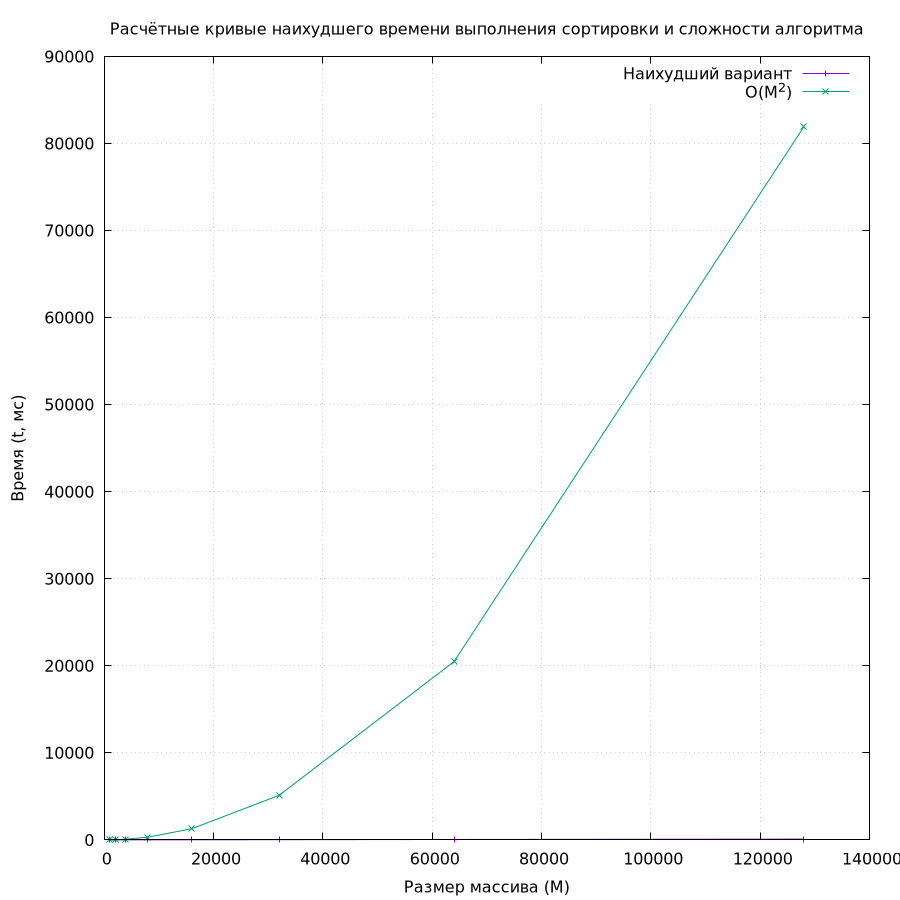
\includegraphics[width=300pt]{worst_and_complexity.png}
	\end{figure}
	\begin{figure}
		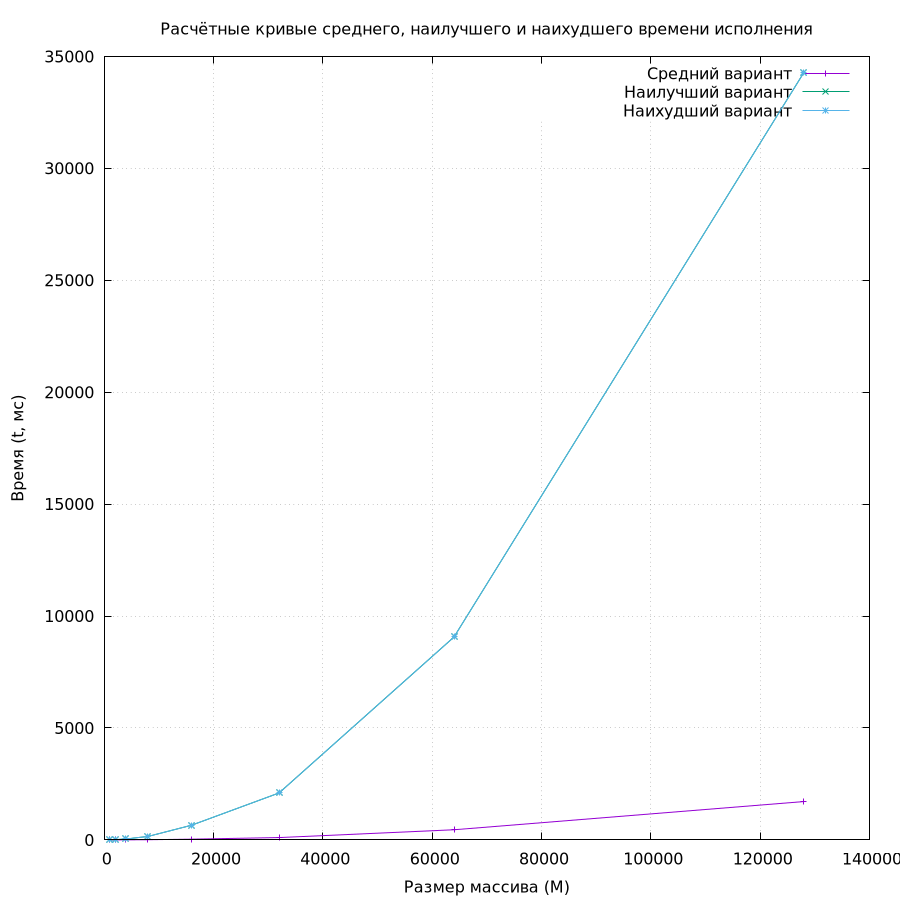
\includegraphics[width=300pt]{average_best_worst.png}
	\end{figure}
	\begin{figure}
		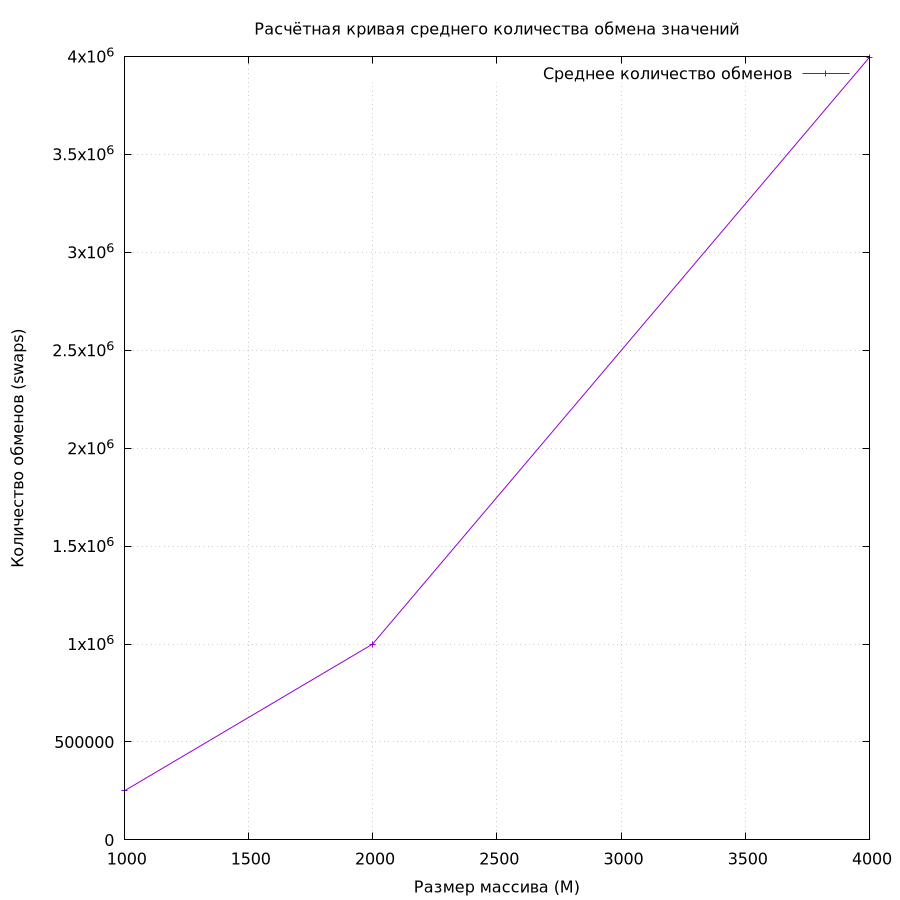
\includegraphics[width=300pt]{average_swaps.png}
	\end{figure}
	\begin{figure}
		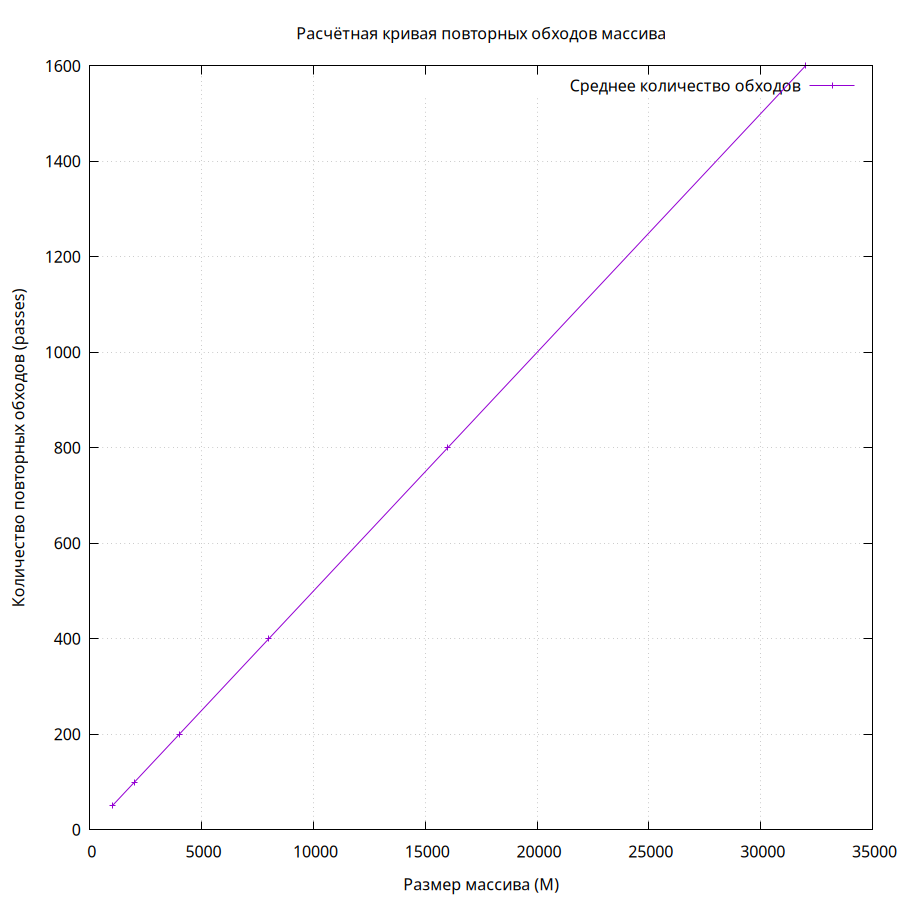
\includegraphics[width=300pt]{average_passes.png}
	\end{figure}

	\vfill
	\clearpage

	\section*{Выводы}
	\addcontentsline{toc}{section}{Выводы}
	Сортировка вставками - простой алгоритм, который имеет временную сложность, равную квадратичной (\( O(N^2) \)). Это означает, что время выполнения алгоритма растёт пропорционально квадрату количества элементов в массиве. Чем больше данных нужно обработать, тем заметнее становится этот эффект. \par
	Данная сортировка наиболее эффективна, когда массив уже частично или полностью упорядочен. В таком варианте количество операций значительно сокращается, и алгоритм работает быстрее. Напротив, если массив отсортирован в обратном порядке, то это наихудший сценарий для данного алгоритма, т.к. количество сравнений и обменов элементов достигает максимума.
\end{document}
